\chapter{Ontologies}

\begin{description}
    \item[Ontology] \marginnote{Ontology} 
        Formal (non-ambiguous) and explicit (obtainable through a finite sound procedure) 
        description of a domain.

    \item[Category] \marginnote{Category}
        Can be organized hierarchically on different levels of generality.

    \item[Object] \marginnote{Object}
        Belongs to one or more categories.

    \item[Upper/general ontology] \marginnote{Upper/general ontology} 
        Ontology focused on the most general domain.

        Properties:
        \begin{itemize}
            \item Should be applicable to almost any special domain.
            \item Combining general concepts should not incur in inconsistencies.
        \end{itemize}

        Approaches to create ontologies:
        \begin{itemize}
            \item Created by philosophers/logicians/researchers.
            \item Automatic knowledge extraction from well-structured databases.
            \item Created from text documents (e.g. web).
            \item Crowd-sharing information.
        \end{itemize}
\end{description}


\section{Categories}
\begin{description}
    \item[Category] \marginnote{Category}
        Used in human reasoning when the goal is category-driven (in contrast to specific-instance-driven).

        In first-order logic, categories can be represented through:
        \begin{descriptionlist}
            \item[Predicate] \marginnote{Predicate categories}
                A predicate to tell if an object belongs to a category 
                (e.g. \texttt{Car(c1)} indicates that \texttt{c1} is a car).

            \item[Reification] \marginnote{Reification}
                Represent categories as objects as well (e.g. $\texttt{c1} \in \texttt{Car}$).
        \end{descriptionlist}
\end{description}

\subsection{Reification properties and operations}
\begin{description}
    \item[Membership] \marginnote{Membership}
        Indicates if an object belongs to a category.
        (e.g. $\texttt{c1} \in \texttt{Car}$).

    \item[Subclass] \marginnote{Subclass}
        Indicates if a category is a subcategory of another one.
        (e.g. $\texttt{Car} \subset \texttt{Vehicle}$).

    \item[Necessity] \marginnote{Necessity}
        Members of a category enjoy some properties 
        (e.g. $(\text{x} \in \texttt{Car}) \Rightarrow \texttt{hasWheels(x)}$).

    \item[Sufficiency] \marginnote{Sufficiency}
        Sufficient conditions to be part of a category\\
        (e.g. $\texttt{hasPlate(x)} \land \texttt{hasWheels(x)} \Rightarrow \texttt{x} \in \texttt{Car}$).

    \item[Category-level properties] \marginnote{Category-level properties}
        Category themselves can enjoy properties\\
        (e.g. $\texttt{Car} \in \texttt{VehicleType}$)

    \item[Disjointness] \marginnote{Disjointness}
        Given a set of categories $S$, the categories in $S$ are disjoint iff they all have different objects:
        \[ \texttt{disjoint($S$)} \iff (\forall c_1, c_2 \in S, c_1 \neq c_2 \Rightarrow c_1 \cap c_2 = \emptyset) \]

    \item[Exhaustive decomposition] \marginnote{Exhaustive decomposition}
        Given a category $c$ and a set of categories $S$, $S$ is an exhaustive decomposition of $c$ iff
        any element in $c$ belongs to at least a category in $S$:
        \[ \texttt{exhaustiveDecomposition($S$, $c$)} \iff \forall o: (o \in c \iff \exists c_2 \in S: o \in c_2) \]

    \item[Partition] \marginnote{Partition}
        Given a category $c$ and a set of categories $S$, $S$ is a partition of $c$ when:
        \[ \texttt{partition($S$, $c$)} \iff \texttt{disjoint($S$)} \land \texttt{exhaustiveDecomposition($S$, $c$)} \]
\end{description}


\subsection{Physical composition}
Objects (meronyms) are part of a whole (holonym).

\begin{description}
    \item[Part-of] \marginnote{Part-of}
        If the objects have a structural relation (e.g. $\texttt{partOf(cylinder1, engine1)}$).

        Properties:
        \begin{descriptionlist}
            \item[Transitivity] $\texttt{partOf(x, y)} \land \texttt{partOf(y, z)} \Rightarrow \texttt{partOf(x, z)}$
            \item[Reflexivity] $\texttt{partOf(x, x)}$
        \end{descriptionlist}

    \item[Bunch-of] \marginnote{Bunch-of}
        If the objects do not have a structural relation.
        Useful to define a composition of countable objects
        (e.g. $\texttt{bunchOf({nail1, nail3, nail4})}$).
\end{description}


\subsection{Measures}

A property of objects.

\begin{description}
    \item[Quantitative measure] \marginnote{Quantitative measure}
        Something that can be measured using a unit\\
        (e.g. $\texttt{length(table1)} = \texttt{cm(80)}$).

        Qualitative measures propagate when using \texttt{partOf} or \texttt{bunchOf} 
        (e.g. the weight of a car is the sum of its parts).

    \item[Qualitative measure] \marginnote{Qualitative measure}
        Something that can be measured using terms with a partial or total order relation
        (e.g. $\{ \texttt{good}, \texttt{neutral}, \texttt{bad} \}$).

        Qualitative measures do not propagate when using \texttt{partOf} or \texttt{bunchOf}.

    \item[Fuzzy logic] \marginnote{Fuzzy logic}
        Provides a semantics to qualitative measures (i.e. convert qualitative to quantitative).
\end{description}


\subsection{Things vs stuff}

\begin{description}
    \item[Intrinsic property] \marginnote{Intrinsic property}
        Related to the substance of the object. It is retained when the object is divided
        (e.g. water boils at 100°C).

    \item[Extrinsic property] \marginnote{Extrinsic property}
        Related to the structure of the object. It is not retained when the object is divided
        (e.g. the weight of an object changes when split).

    \item[Substance] \marginnote{Substance}
        Category of objects with only intrinsic properties.

        \begin{description}
            \item[Stuff] \marginnote{Stuff}
                The most general substance category.
        \end{description}

    \item[Count noun] \marginnote{Count noun}
        Category of objects with only extrinsic properties.

        \begin{description}
            \item[Things] \marginnote{Things}
                The most general object category.
        \end{description}
\end{description}



\section{Semantic networks}
\marginnote{Semantic networks}
Graphical representation of objects and categories connected through labeled links.

\begin{figure}[H]
    \centering
    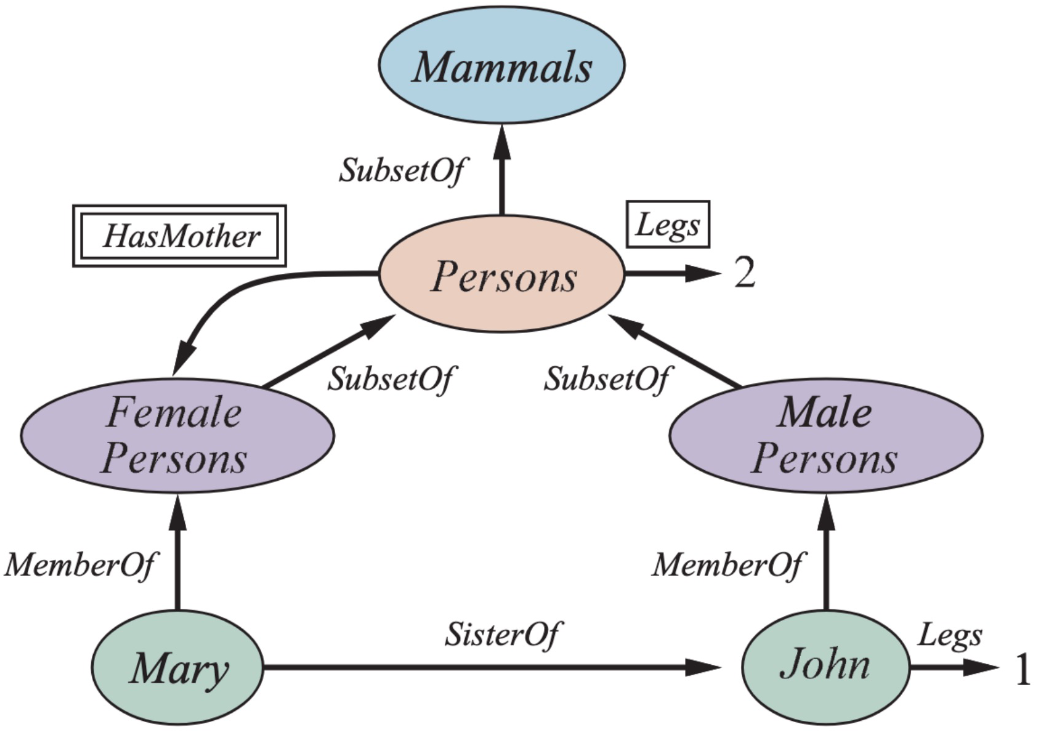
\includegraphics[width=0.4\textwidth]{img/semantic_network.png}
    \caption{Example of semantic network}
\end{figure}

\begin{description}
    \item[Objects and categories] Represented using the same symbol.

    \item[Links] Four different types of links:
        \begin{itemize}
            \item Relation between objects (e.g. \texttt{SisterOf}).
            \item Property of a category (e.g. 2 \texttt{Legs}).
            \item Is-a relation (e.g. \texttt{SubsetOf}).
            \item Property of the members of a category (e.g. \texttt{HasMother}).
        \end{itemize} 
\end{description}

\begin{description}
    \item[Single inheritance reasoning] \marginnote{Single inheritance reasoning}
        Starting from an object, check if it has the queried property.
        If not, iteratively move up to the category it belongs to and check for the property.

    \item[Multiple inheritance reasoning] \marginnote{Multiple inheritance reasoning}
        Reasoning is not possible as it is not clear which parent to choose.
\end{description}

\begin{description}
    \item[Limitations]
        Compared to first-order logic, semantic networks do not have:
        \begin{itemize}
            \item Negations.
            \item Universally and existentially quantified properties.
            \item Disjunctions.
            \item Nested function symbols.
        \end{itemize}

        Many semantic network systems allow to attach special procedures to handle special cases 
        that the standard inference algorithm cannot handle.
        This approach is powerful but does not have a corresponding logical meaning.

    \item[Advantages]
        With semantic networks, it is easy to attach default properties to categories and
        override them on the objects (i.e. \texttt{Legs} of \texttt{John}).
\end{description}



\section{Frames}
\marginnote{Frames}
Knowledge that describes an object in terms of its properties.
Each frame has:
\begin{itemize}
    \item A unique name
    \item Properties represented as pairs \texttt{<slot - filler>}
\end{itemize}

\begin{example}
    \phantom{}\\[-1em]
    \begin{lstlisting}[mathescape=true, language={}] 
        (
            toronto
                <:Instance-Of City>
                <:Province ontario>
                <:Population 4.5M>
        )
    \end{lstlisting}
\end{example}

\begin{description}
    \item[Prototype] \marginnote{Prototype}
        Members of a category used as comparison metric to determine if another object belongs to the same class
        (i.e. an object belongs to a category if it is similar enough to the prototypes of that category).

    \item[Defeasible value] \marginnote{Defeasible value}
        Value that is allowed to be different when comparing an object to a prototype.

    \item[Facets] \marginnote{Facets}
        Additional information contained in a slot for its filler (e.g. default value, type, domain).

        \begin{description}
            \item[Procedural information] 
                Fillers can be a procedure that can be activated by specific facets:
                \begin{descriptionlist}
                    \item[\texttt{if-needed}] Looks for the value of the slot.
                    \item[\texttt{if-added}] Adds a value.
                    \item[\texttt{if-removed}] Removes a value.
                \end{descriptionlist}
                \begin{example}
                    \phantom{}\\[-1em]
                    \begin{lstlisting}[mathescape=true, language={}] 
    (
        toronto
            <:Instance-Of City>
            <:Province ontario>
            <:Population [if-needed QueryDB]>
    )
                    \end{lstlisting}
                \end{example}
        \end{description}
\end{description}